\begin{enumerate}[label=\thechapter.\arabic*,ref=\thechapter.\theenumi]
\item Let y\brak{t}=x\brak{4t},where x\brak{t} is a continous-time periodic signal of $100$s.the fundamental period of y\brak{t} is (\textbf{rounded off to the nearest integer})
 \hfill(GATE IN 2023)\\
\solution
\input{2023/IN/29/assign4.tex}
\newpage

\item In the circuit shown below, it is observed that the amplitude of voltage across the resistor is the same as the amplitude of the sorce voltage. What is the angular frequency $\omega_0$(in rad$/s$)?\\
\begin{circuitikz}[american]
    \draw (0,0) to[R, l=$10K\Omega$] (2,0) to[L, l=$10mH$] (4,0) to[C, l=$1\mu{F}$] (6,0) -- (6,-1) 
    to[sV, l=$100\cos(\omega_0 t)$] (0,-1) -- (0,0)
    (0,-1) node[circ]{} node[left]{$+$}
    (6,-1) node[circ]{} node[right]{$-$};
\end{circuitikz}
\begin{enumerate}
    \item[(A)] $10^4$\\
    \item[(B)] $10^3$\\
    \item[(C)] $10^3\pi$\\
    \item[(D)] $10^4\pi$  
\end{enumerate} \hfill(GATE BM 2023)\\
\solution
\iffalse
\let\negmedspace\undefined
\let\negthickspace\undefined
\documentclass[journal,12pt,twocolumn]{IEEEtran}
\usepackage{cite}
\usepackage{amsmath,amssymb,amsfonts,amsthm}
\usepackage{algorithmic}
\usepackage{graphicx}
\usepackage{textcomp}
\usepackage{xcolor}
\usepackage{txfonts}
\usepackage{listings}
\usepackage{enumitem}
\usepackage{mathtools}
\usepackage{gensymb}
\usepackage{comment}
\usepackage{tikz}
\usepackage[breaklinks=true]{hyperref}
\usepackage{tkz-euclide} 
\usepackage{listings}
\usepackage{gvv}
\def\inputGnumericTable{}
\usepackage[latin1]{inputenc}                              
\usepackage{color}                                            
\usepackage{array}                                            
\usepackage{longtable}                                       
\usepackage{calc}                                             
\usepackage{multirow}   
\usetikzlibrary{circuits.ee.IEC}
\usepackage{hhline}                                           
\usepackage{ifthen} 
\usepackage{circuitikz}
\usepackage{lscape}
\newtheorem{theorem}{Theorem}[section]
\newtheorem{problem}{Problem}
\newtheorem{proposition}{Proposition}[section]
\newtheorem{lemma}{Lemma}[section]
\newtheorem{corollary}[theorem]{Corollary}
\newtheorem{example}{Example}[section]
\newtheorem{definition}[problem]{Definition}
\newcommand{\BEQA}{\begin{eqnarray}}
\newcommand{\EEQA}{\end{eqnarray}}
\newcommand{\define}{\stackrel{\triangle}{=}}
\theoremstyle{remark}
\newtheorem{rem}{Remark}
\begin{document}

\bibliographystyle{IEEEtran}
\vspace{3cm}

\title{GATE-2023 BM Q-42}
\author{EE23BTECH11207 -KAILASH.C$^{*}$% <-this % stops a space
}
\maketitle
\newpage
\bigskip

\renewcommand{\thefigure}{\theenumi}
\renewcommand{\thetable}{\theenumi}
In the circuit shown below, it is observed that the amplitude of voltage across the resistor is the same as the amplitude of the sorce voltage. What is the angular frequency $\omega_0\brak{in rad/s}$?
\begin{circuitikz}[american]
    \draw (0,0) to[R, l=$10K\Omega$] (2,0) to[L, l=$10mH$] (4,0) to[C, l=$1\mu{F}$] (6,0) -- (6,-1) 
    to[sV, l=$100\cos\brak{\omega_0 t}$] (0,-1) -- (0,0)
    (0,-1) node[circ]{} node[left]{$+$}
    (6,-1) node[circ]{} node[right]{$-$};
\end{circuitikz}

\begin{enumerate}
    \item[(A)] $10^4$\\
    \item[(B)] $10^3$\\
    \item[(C)] $10^3\pi$\\
    \item[(D)] $10^4\pi$  
\end{enumerate} \hfill(GATE 2023 BM)
\solution
\fi

\begin{table}[h]
\begin{tabular}{|l|l|l|}
\hline
\textbf{Symbols} & \textbf{Parameters} & \textbf{Value}\\ \hline
R & Resistance & $10K\Omega$ \\ \hline
L & Inductance & $10mH$ \\ \hline
C & Capacitance & $1\mu{F}$\\ \hline
$\omega_0$ & Angular Frequency & \\ \hline
$V_s$ & Source Voltage & \\ \hline
\end{tabular}
\caption{Parameter Table}
\label{tab:gate.bm.42}
\end{table}
\\
\begin{circuitikz}[american]
    \draw (0,0) to[R, l=$10K\Omega$] (2,0) to[L, l=$10^{-2}j\omega_0$] (4,0) to[C, l=$\frac{10^6}{j\omega_0}$] (6,0) -- (6,-1) 
    to[sV, l=$100\cos\brak{\omega_0 t}$] (0,-1) -- (0,0)
    (0,-1) node[circ]{} node[left]{$+$}
    (6,-1) node[circ]{} node[right]{$-$};
\end{circuitikz}

We have:
\begin{align}
    V_R&=V_s \label{eq:421}
\end{align}
Using KVL:
\begin{align}
    V_s&=V_R+V_C+V_L\label{eq:422}
\end{align}
By using \eqref{eq:421} in \eqref{eq:422}:
\begin{align}
    V_C&=-V_L\label{eq:423}\\
    X_C&=-X_L\label{eq:424}\\
    \frac{1}{j\omega_0C}&=-j\omega_0L\label{eq:425}\\
\frac{1}{LC} &= -j^2\omega_0^{2} \label{eq:426}\\ 
\omega_0^{2}&=\frac{1}{LC}\label{eq:427}\\
\omega_0&=\frac{1}{\sqrt{LC}} \label{eq:428}\\
&=\frac{1}{\sqrt{10^{-2}\times10^{-6}}}\label{eq:429}\\
&=\frac{1}{10^{-4}}\label{eq:4210}\\
&=10^4 rad/s\label{eq:4211}
\end{align}
\begin{figure}[h]
        \centering
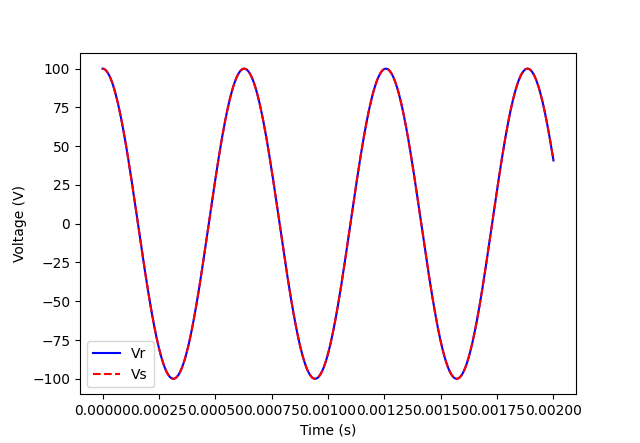
\includegraphics[width=\columnwidth]{2023/BM/42/figs/Figure42.png}
    \caption{Voltage across Resistor and Source voltage}
    \label{fig:plot42}
\end{figure}

\newpage

\item For a regular sinusoidal wave propagating in deep water having wave height of 3.5 m and wave period of 9 s, the wave steepness is \underline{\hspace{1cm}} (round off to three decimal places).
\hfill Gate 2023 NM 33\\
\solution
\input{2023/NM/33/g2.tex}
\newpage

\item  A spring mass system is shown in the figure . Take the value of acceleration  due to gravity as $g=9.81m/s^2$.The static deflection due to weight and the time period of the oscillations,respectively,are\\
 \begin{figure}[h!]
    \centering
    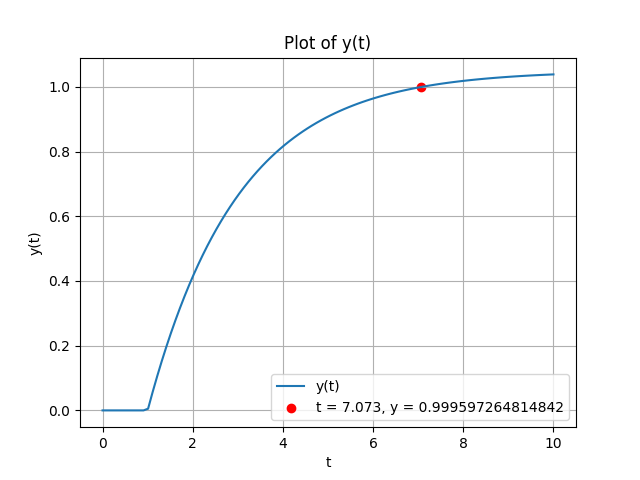
\includegraphics[width = \columnwidth]{2023/XE/71/figs/fig1.jpg}
\end{figure}
\hfill{(GATE 2023 XE)}\\
\solution
\input{2023/XE/71/assignment5.tex}
\pagebreak

\item In the circuit shown below, the amplitudes of the voltage across the resistor and the capacitor are equal. What is the value of the angular frequency $\omega_o$ (in rad/s)? 
(Round off the answer to one decimal place.) \hfill(GATE BM 32 2023)
\begin{circuitikz}
    % Voltage source
    \draw (0,0) to[sV, v=$100\cos(\omega_{o} t)$] (0,2);
    
    % Resistor
    \draw (0,2) to[R, l=$1\text{ k}\Omega$] (3,2);
    
    % Capacitor
    \draw (3,2) to[C, l=$100\mu\text{F}$] (3,0);
    
    % Ground
    \draw (3,0) -- (0,0);
\end{circuitikz}
\solution
\iffalse
\let\negmedspace\undefined
\let\negthickspace\undefined
\documentclass[journal,12pt,twocolumn]{IEEEtran}
\usepackage{cite}
\usepackage{amsmath,amssymb,amsfonts}
\usepackage{graphicx}
\usepackage{textcomp}
\usepackage{xcolor}
\usepackage{txfonts}
\usepackage{listings}
\usepackage{enumitem}
\usepackage{mathtools}
\usepackage{gensymb}
\usepackage{comment}
\usepackage[breaklinks=true]{hyperref}
\usepackage{tkz-euclide} 
\usepackage{listings}
\usepackage{gvv}                                        
\def\inputGnumericTable{}                                 
\usepackage[latin1]{inputenc}                                
\usepackage{color}                                            
\usepackage{array}                                            
\usepackage{longtable}                                       
\usepackage{calc}                                             
\usepackage{multirow}                                         
\usepackage{hhline}                                           
\usepackage{ifthen}                                           
\usepackage{lscape}
\usepackage[export]{adjustbox}

\newtheorem{theorem}{Theorem}[section]
\newtheorem{problem}{Problem}
\newtheorem{proposition}{Proposition}[section]
\newtheorem{lemma}{Lemma}[section]
\newtheorem{corollary}[theorem]{Corollary}
\newtheorem{example}{Example}[section]
\newtheorem{definition}[problem]{Definition}
\newcommand{\BEQA}{\begin{eqnarray}}
\newcommand{\EEQA}{\end{eqnarray}}
\newcommand{\define}{\stackrel{\triangle}{=}}
\newtheorem{rem}{Remark}

\begin{document}
\parindent 0px
\bibliographystyle{IEEEtran}

\vspace{3cm}

\title{}
\author{EE23BTECH11042 -  Khusinadha Naik$^{*}$
}
\maketitle
\newpage
\bigskip

% \renewcommand{\thefigure}{\theenumi}
% \renewcommand{\thetable}{\theenumi}


\noindent \textbf{26.} \hspace{2pt}A causal, discrete time system is described by the difference equation $y[n] = 0.5 y[n-1] + x[n]$, for all $n$, where $y[n]$ denotes the output sequence and $x[n]$ denotes the input sequence. Which of the following statements is/are TRUE?
\begin{flushright}
\hfill(GATE 2023 BM)
\end{flushright}
\begin{enumerate}[label = (\alph*)]
	\item The system has an impulse response described by $0.5^{n} u[-n]$ where $u[n]$ is the  
unit step sequence. 	\label{option:GATE.2023.BM.26.1}	
	\item The system is stable in the bounded input, bounded output sense.		\label{option:GATE.2023.BM.26.2}
	\item The system has an infinite number of non-zero samples in its impulse response	\label{option:GATE.2023.BM.26.3}
	\item The system has a finite number of non-zero samples in its impulse response.	\label{option:GATE.2023.BM.26.4}
\end{enumerate}

\noindent \textbf{Ans.}\\
\fi
\begin{table}[h]
\centering
\begin{tabular}{|c|c|c|}
        \hline
        \textbf{Parameter} & \textbf{Value} & \textbf{Description} \\
        \hline
        $x[n]$ & ? & Input Sequence \\
        \hline
        $y[n]$ & ? & Output Sequence \\
        \hline
\end{tabular}
\caption{Input parameters table}
\label{tab:GATE.2023.BM.26.1}





\end{table}
\begin{align}
y[n] = 0.5y[n-1] + x[n] 
\end{align}

Taking $Z$-Transform 
\begin{align}
Y\brak{z} &= 0.5z^{-1}Y\brak{z} + X\brak{z} \\
\implies \frac{Y\brak{z}}{X\brak{z}} &= \frac{1}{1 - 0.5z^{-1}} = H\brak{z} 
\end{align}
If $x[n]$ is impulse input 
\begin{align}
\implies &Y\brak{z} = H\brak{z} = \frac{1}{1 - 0.5z^{-1}}  \label{eq:GATE.2023.BM.26.4}
\end{align}
From \eqref{eq:GATE.2023.BM.26.4} pole lies at $z = 0.5$
\begin{align}
a^{n}u\brak{n} \xleftrightarrow{\mathcal{Z}} &\frac{1}{1 - az^{-1}} \quad , \abs{z} > a \label{eq:GATE.2023.BM.26.5}
\end{align}

From \eqref{eq:GATE.2023.BM.26.4} , \eqref{eq:GATE.2023.BM.26.5}
\begin{align}
h[n] = 0.5^{n}u[n] \quad , \abs{z} > 0.5 \label{eq:GATE.2023.BM.26.6}
\end{align}


\pagebreak
Plotting $h[n]$ vs $n$
\begin{figure}[h]
    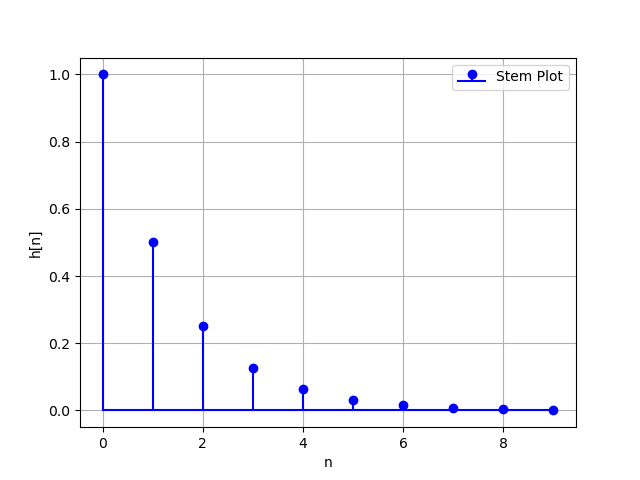
\includegraphics[width=0.5\textwidth]{2023/BM/26/figs/fig1.png}
    \caption{Plot of $h[n]$ vs $n$}
    \label{fig:GATE.2023.BM.26.1}
\end{figure}

\begin{enumerate}
\item From \eqref{eq:GATE.2023.BM.26.6} , \ref{option:GATE.2023.BM.26.1} is wrong
\item As pole lies within unit circle \ref{option:GATE.2023.BM.26.2} is true
\item From \eqref{eq:GATE.2023.BM.26.6} and \figref{fig:GATE.2023.BM.26.1} ,\ref{option:GATE.2023.BM.26.3} is true and hence
\item \ref{option:GATE.2023.BM.26.4} is false 
\end{enumerate}





%\end{document}

\pagebreak
\item Let $ w ^{4} = 16j $. Which of the fo
    llowing can not be the value of w?\\\
    \
 52 (A)   $2e^\frac{j2 \pi}{8}$\\
 53 (B)   $2e^\frac{j \pi}{8}$\\
 54 (C)   $2e^\frac{j5 \pi}{8}$\\
 55 (D)   $2e^\frac{j9 \pi}{8}$\\
\hfill{(GATE 2023 EC)}\\               \solution                              \input{2023/EC/13/gateec131.tex}     \pagebreak
\end{enumerate}
